\section{Results}




\subsection{Periodic}



\begin{figure}[htp]
  \centering
  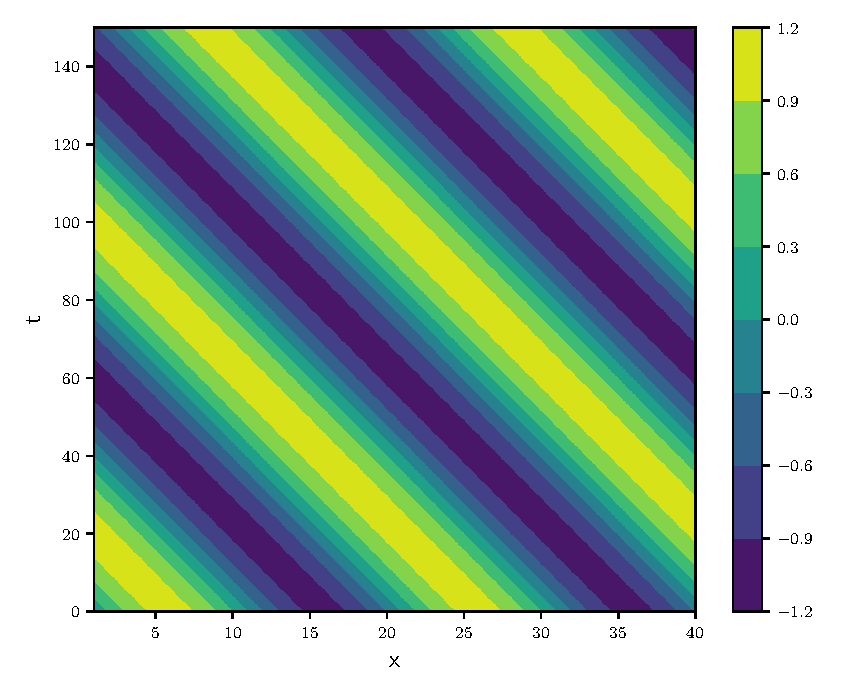
\includegraphics[width=\textwidth]{../figures/psi_periodic_centered_short.pdf}
  \caption{Hovmuller diagram for the periodic domain with a sinusoidal initial
  state using a central difference in time. Waves propagate westward.}
  \label{fig:periodic_sine}
\end{figure}


\begin{figure}[htp]
  \centering
  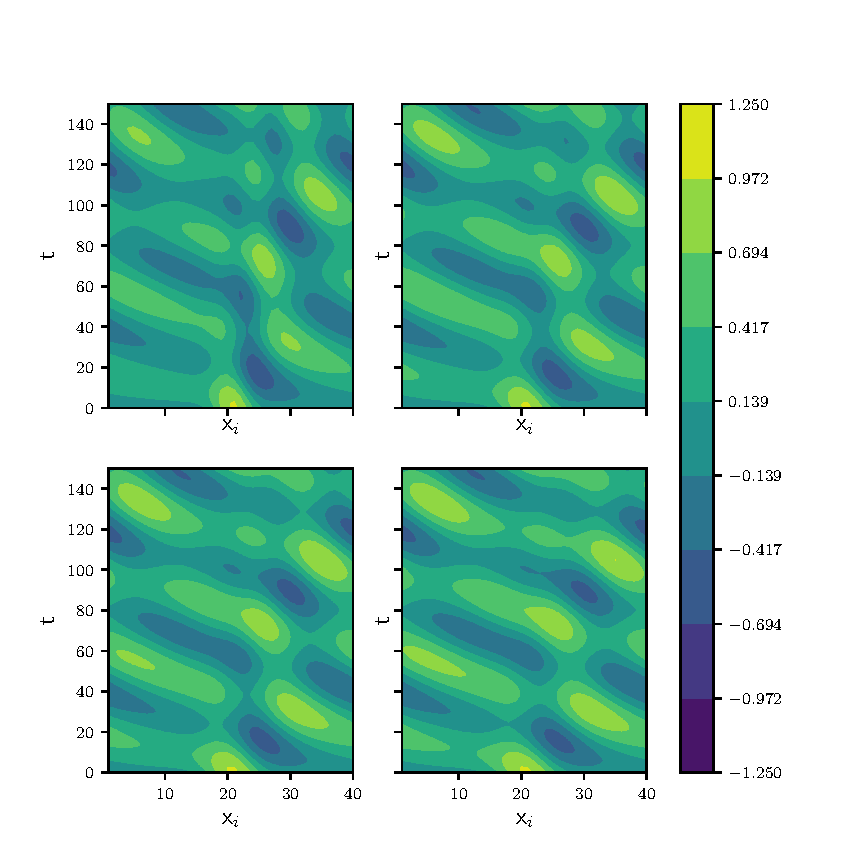
\includegraphics[width=\textwidth]{../figures/hovmuller_sigma.pdf}
  \caption{Hovmuller diagram for the periodic domain with a gaussian initial
  state.
  From top left to bottom right: $\sigma = \brak{0.08, 0.10, 0.11, 0.12}$.
  }
  \label{fig:periodic_gauss}
\end{figure}



\subsection{Bounded}

\begin{figure}[htp]
  \centering
  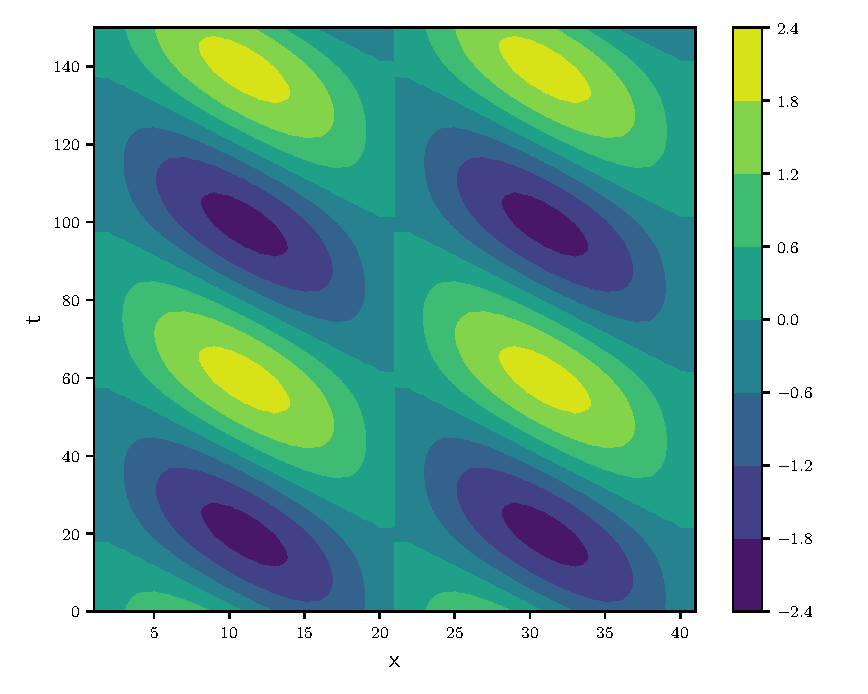
\includegraphics[width=\textwidth]{../figures/psi_bounded_centered_sine.pdf}
  \caption{Hovmuller diagram for the bounded domain with a sinusoidal initial
  state.}
  \label{fig:bounded_sine}
\end{figure}


\begin{figure}[htp]
  \centering
  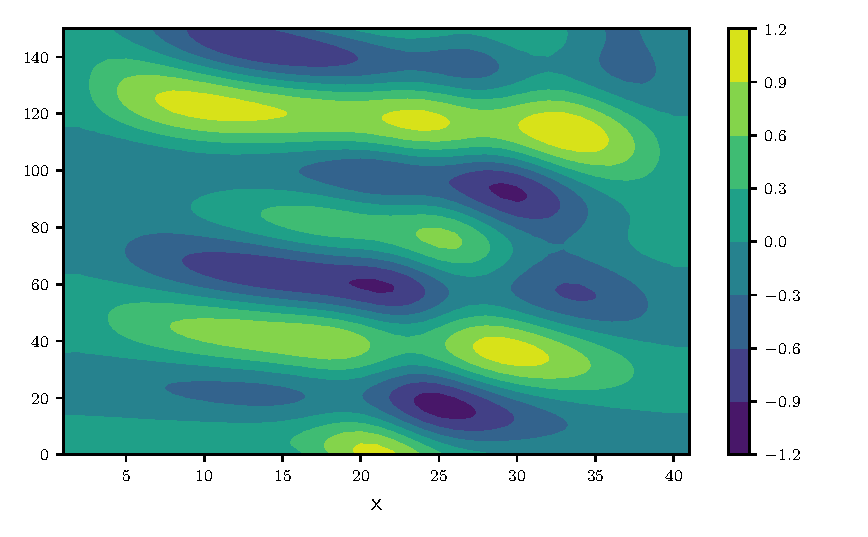
\includegraphics[width=\textwidth]{../figures/psi_bounded_centered_gauss.pdf}
  \caption{Hovmuller diagram for the bounded domain with a gaussian initial
  state.}
  \label{fig:bounded_gauss}
\end{figure}


\subsection{Phase speed}


Looking at the hovmuller diagrams for the periodic case we
can extract the phase speed as 1/160 = 0.00625.
For the bounded we use 1/(100 - 20) = 0.0125.
